%\chapter{Introduction to ADCs}\label{ap:primer}
Today we can place more than a billion transistor (1 000 000 000) on a
chip. The majority of transistors are used for digital processing and all  digital
processing needs input. 

If the 
input is already digital --- a digital photograph, a music file, an
excel sheet, or a video clip --- the chip can start processing
right away. If the information is from the real world --- the output
from a crash accelerometer, a video signal, a radio signal, a signal
from a microphone,
the signal from an ultrasound probe, or the signal from a
electrocardiogram (ECG) --- it must be converted
to digital. 

The real world is analog --- continuous in time and
continuous in value. If you move your arm up and down you will
  notice that it does not jump from one place to another, but move in
  a continuous motion. This is continuous in value. Continuous in time
  means that the movement is not a sequence of snapshots.

 Digital information is discrete in time and
discrete in value. If you move your arm up and down in a
  digital world, the arm will jump from one point to another, and it
  will be impossible to place it between two points. In addition, the
  arm will only jump at specified times.

To convert information from analog to digital we use an
analog-to-digital converter (ADC). The ADC turns continuous time to
discrete time, and continuous value to discrete value.

The ADC
divide the continuous values into a number of discrete levels. It's like
rounding a floating point number (1.1 or 1.1204058) to an integer
(1). The number of levels in an ADC are specified by the number of
bits (B). A 6-bit ADC has $2^6 = 64$ levels and a 16-bit ADC has
$2^{16} = 65536$ levels. The number of levels is called the resolution
and determine the accuracy. ADCs range from 1-bit
resolution to 24-bit resolution.

The ADC turns continuous time into discrete time by sampling. Think of
a Black Moor (a goldfish) swimming back and forth in an aquarium. You have marked 32
points on the glass to mark the horizontal position. At the beat of
a metronome you write down where the fish is. That is sampling,
only measuring something at timed intervals. 

In an ADC the intervals are
determined by the sampling frequency, written in samples per second
(S/s). ADCs range from 1S/s to 40GS/s (40 000 000 000
samples per second). 

It would be nice to have a single 24-bit 40GS/s ADC to cover all
applications, but it can't be done. Not because we don't know how
to do it, but because the Heisenberg Uncertainty Principle says it's
impossible \cite{walden99}. Even if it could be done we would not want
to because a 24-bit 40GS/s ADC will consume 2.8 million watts
\footnote{
The required capacitance is given by
\eqn{
C =  \dfrac{48 k T 2^{2B}}{V_{PP}^2}  
}
where $k$ is Boltzmann's constant, $T$ is the temperature in Kelvin,
$B$ is the number of bits, and $V_{PP}$ is the peak-to-peak signal
swing.


 If we assume a
transconductance amplifier, it needs a transconductance of
\eqn{
  g_m = 2 \pi C f_s
}
And a current of 
\eqn{
  I = \half gm \times V_{EFF}
}
where $V_{EFF}$ is the effective overdrive of the transistor that
provides the transconductance.

If we assume $V_{EFF} = V_{DD}/10$, $V_{PP} = \half V_{DD}$, and $P =
V_{DD} I$, where $P$ is the power dissipation we have that
\eqn{
 P = 19.2 \pi k T 2^{2B} f_s
}
which for $B=24$, $T=300$ and $f_s=40GHz$ is $P=2.8MW$
}, 500 times more than an
electric stove. At that power dissipation my cellphone battery would
last 3.6ms (0.0036 s).\footnote{My cellphone battery has
  780mAh. With a current drain of $I= P/V = 2.8MW/3.6V = 778kA$ it
  would run for $780mAh/778kA = 3.6 ms$.}

%This thesis cover two
%types of ADCs: medium resolution (8-bit) high speed (60MS/s) ADC, and
%high resolution (15-bit) high speed ($>$ 10MS/s) ADC. The first type is
%used in digital communications, digital storage read channels and
%medical imaging. The second type is used in ultrasound equipment,
%IF sampling recievers, and battery powered instruments. 
This paper give an introduction to ADCs and is organized as follows:
Section \ref{sc:adc_limits} cover noise and distortion phenomena in
ADC converter. Section \ref{sc:adc_measures} detail the measures and
abbreviations used when talking about ADCs. In Section
\ref{sc:adc_pipelined} we discuss one of ADC architectures featured in
this thesis, the pipelined ADC.

For
a deeper introduction to data converters we suggest reading
\cite{johns}, or \cite{plassche}. 



\section{Limiting factors for ADC accuracy}\label{sc:adc_limits}
%#####################################################################
\subsection{Noise}
%#####################################################################
Noise is present in any analog system. Noise sources are often divided into two categories: {\em
  intrinsic} and {\em extrinsic}. {\em Intrinsic} refer to an
inherent property of the system. {\em Extrinsic} refers to an external
influence. In this section we will describe the {\em
  Intrinsic} phenomena of noise.

Noise manifests as random fluctuation of a signal. 
There are three main noise sources: thermal noise, shot noise and
flicker noise. Thermal noise stem from the random fluctuation of
charge carriers, shot noise from charge carriers moving across a
potential barrier and flicker noise from the random trapping and release
of charge carriers. Thermal noise and flicker noise are the dominating
noise sources in MOSFET transistors. The dominating noise source in
high-speed analog-to-digital converters (ADCs) is thermal
noise. For a comprehensive treatise on noise phenomena we refer to Aldert Van Der
Ziel's ``Noise in Solid State Devices and Circuits'' \cite{ziel}.

Noise place a lower limit on the resolution of a system. The systems
discussed in this thesis are switched-capacitor circuits which have an
accumulated noise approximated by
\eqn{
  V_n^2 = a_1 kT/C
}
where $k$ is Boltzmann's constant ($1.38\times10^{-23}$), $T$ the
temperature in Kelvin, $C$ the sampling capacitance and $a_1$ a
constant. 


%#####################################################################
\subsection{Quantization errors}
%#####################################################################
One of the fundamental limitations of Nyquist converters is the
quantization error. Quantization of a continuous value signal is a non-linear
operation. We  define the output $y_Q$ as 
\eqn{
\label{eq:quantizer}
  y_Q = Q(y_a) = y_a + q_e
}
where $y_a$ is the input signal, $Q(x)$ is the quantization function and
$q_e$ is the error signal due to quantization.

\subsubsection{The exact solution}
The quantization operation distort the input signal.  We can write
the quantization error, $q_e$,  as 
\eqn{
 q_e = y_{a} - y_{Q} 
}
If the input signal, $y_a$, is a ramp function, the quantization error will be a
sawtooth function. 

%Using a sinusoid as the
%input signal, the quantization error becomes more complex, and can be
%written as
%\eqn{
%q_e = A sin(\omega t)\left(1 - \frac{1}{2 |A sin(\omega t)|} \right)
%}
%for a 1-bit converter.
For a sinusoidal input the quantization error become more complex.
For the N-bit case the quantization error can be written as \cite{blachman85}
\eqn{
\label{eq:blachout}
  y_Q = \sum_{p=1}^\infty{A_p\sin{p\omega t}}
}
where $\omega$ is the angular frequency,
$t$ is time and $p$ is the harmonic index. The amplitude of the
individual harmonics, $A_p$, is defined as 
\eqna{
\label{eq:apone}
A_p &{}={}& \delta_{p1}A  + \sum_{m =
  1}^\infty{\frac{2}{m\pi}J_p(2m\pi A)}, p = odd \\
A_p  &{}={}& 0, p = even
}
where
\eqna{
\delta_{p1} = 1,  p=1\\
\delta_{p1} = 0, p \neq 1
}and $J_p(x)$ is a Bessel function of the first kind. 
If we approximate the amplitude of the input signal as
\eqn{
A = \frac{2^n - 1}{2} \approx 2^{n-1}
}
where n is the number of bits, we can rewrite \req{apone} as 
\eqn{
\label{eq:aptwo}
A_p = \delta_{p1}2^{n-1} + \sum_{m=1}^\infty{\frac{2}{m\pi}J_p(2m\pi
  2^{n-1})},  p=odd
}

Quantization error only contain odd harmonics of the input signal. The
expression in \req{aptwo} is complex to calculate, and is not suited
for a quick approximation of the quantization error.

%---------------------------------------------------------------------
\subsubsection{The approximation}
%---------------------------------------------------------------------
It is generally accepted that for sufficient quantization steps
(enough bits) and an active input signal the quantization error, $q_e$,
can be approximated by a white noise \cite{widrow56}.
The quantization error varies between $-\frac{1}{2}LSB < q_e <
\frac{1}{2}LSB$ and has an average power of $\overline{q_e^2} =
\frac{1}{12}LSB^2$. The quantization error place a
fundamental limit of the resolution of a Nyquist converter with a
finite number of bits. The general expression of signal to noise ratio is
\eqn{
\label{eq:snrcom}
SNR = 6.02 B + 1.76 dB
}
where $B$ is the number of bits and we assume a sinusoidal input signal.

%---------------------------------------------------------------------
\subsubsection{The exact solution versus the approximation}
%---------------------------------------------------------------------

A more accurate expression for the dynamic range than \req{snrcom} of a n-bit
converter, derived from \req{blachout} and \req{aptwo}, is
\eqn{
\label{eq:snraccurate}
SNR = \frac{2^{n-1} +
  \sum_{m=1}^\infty{\frac{2}{m\pi}J_1(2m\pi2^{n-1})}}{
\sqrt{\sum_{i=1}^\infty{[\sum_{m=1}^\infty{\frac{2}{m\pi}J_{2i+1}(2m\pi2^{n-1})}]^2}}}
}

In Table \ref{tab:snr_accurate_vs_approximation} the SNR for 1 to 10
bits in the quantizer is shown \cite{plassche}. The approximation \req{snrcom}
overestimates the signal-to-noise ratio. The overestimation is reduced
with a higher number of bits.

\begin{table}[ht]
\centering 
\begin{tabular}{c|c|c|r}
\label{tab:snr_accurate_vs_approximation}
Number of bits&Accurate SNR&Approximate SNR&Percent error\\
\hline 
1&6.31&7.78 & 18\%\\
2&13.30&13.80 & 6\% \\
3&19.52&19.82 & 3.5\%\\
4&25.59&25.84 & 2.9\%\\
5&31.65&31.86 & 2.4\%\\
6&37.70&37.88 & 2\%\\
7&43.76&43.90 & 1.6\%\\
8&49.82&49.92 & 1.1\%\\
9&55.87&55.94 & 0.8\%\\
10&61.93&61.96 & 0.3\%
\end{tabular}
\caption{SNR as function of the number of bits.}
\end{table}

\subsection{Sampling clock jitter}
Sampling is
controlled by a clock signal. The clock signal has a frequency ($f_s$)
called the sampling frequency. According to the sampling theorem \cite{shannon49}, signal frequencies at, or below,
$\half{f_s}$ can be accurately reproduced from the sampled
data. 

How accurate a signal can be sampled depend on the sampling time
uncertainty called jitter or
clock phase noise. Jitter is a
random fluctuation of the sampling instance. The source of jitter is
usually thermal noise in clock buffer-, amplifier- or
generator-circuits \cite{plassche}. 

The effect of jitter is more noise. The results can
be seen in \reg{jit_fft} and \reg{jit_time}. In \reg{jit_fft} the sampled spectrum with and without jitter
is shown. Note that the signal without jitter has finite resolution
because we have added noise to emulate quantization noise. 
The
jitter is simulated as a random fluctuation of the
sampling instant. From 
\reg{jit_fft} we can see that noise power is increased when jitter
is added. In \reg{jit_time}, signals are shown in time
domain. We can see that the signal with jitter samples an incorrect value
from the input signal. 
\begin{figure}[!htb]
\centering 
 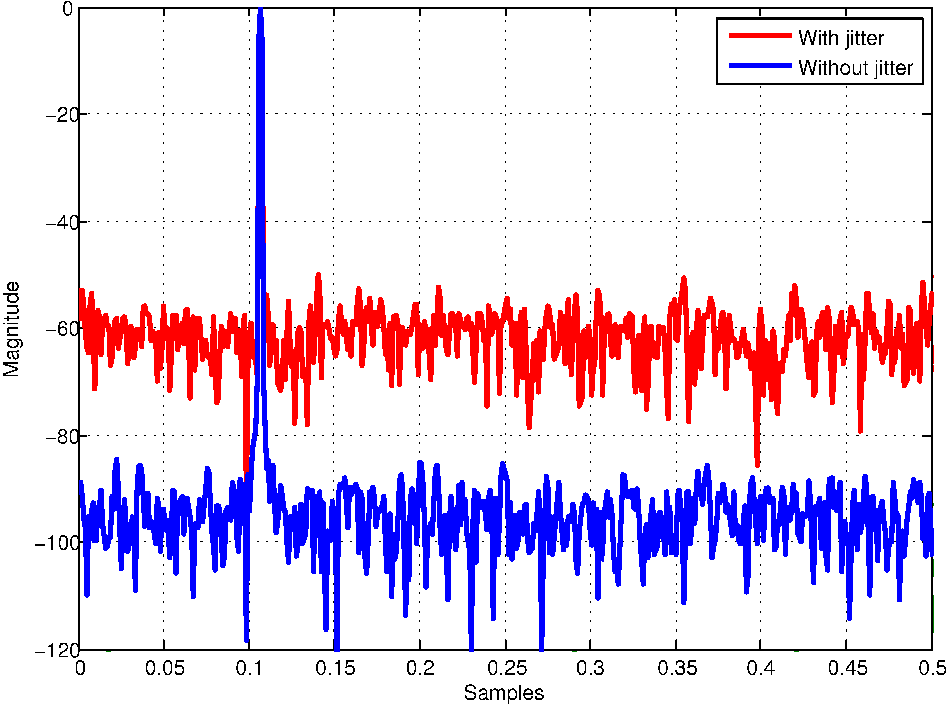
\includegraphics[width=\myfigwidth]{graphics/jit_fft}
  \caption{Spectrum with and without jitter in sampling of a sinusoid}
  \label{fig:jit_fft}
\end{figure}

\begin{figure}[!htb]
\centering 
 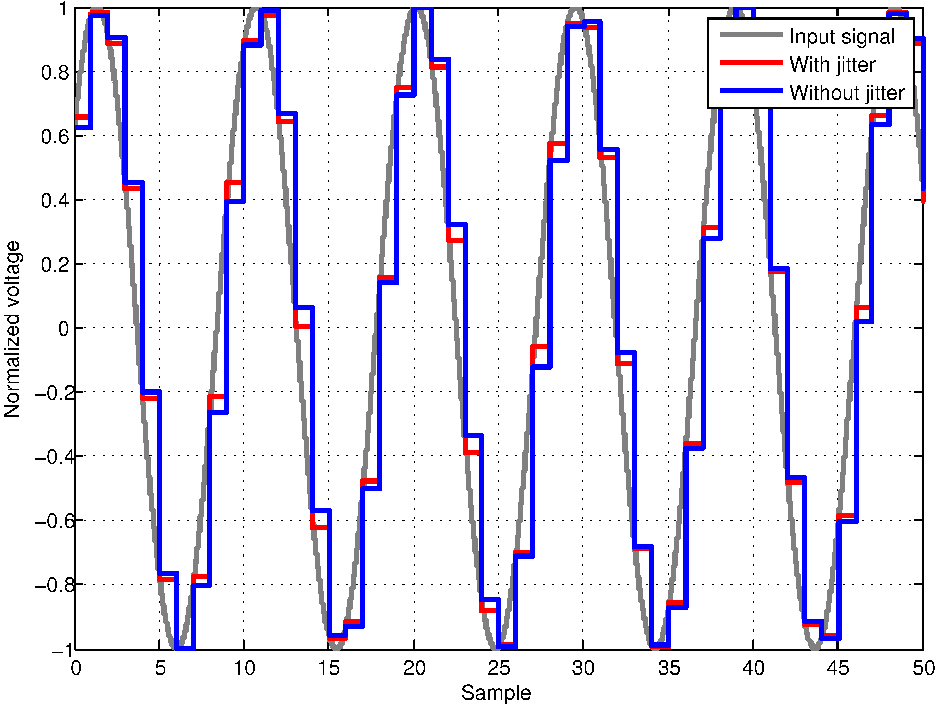
\includegraphics[width=\myfigwidth]{graphics/jit_time}
  \caption{Time domain plot with and without jitter in sampling of a sinusoid}
  \label{fig:jit_time}
\end{figure}

It is possible to derive equations for the maximum jitter that can be
tolerated in an ADC. As we can see from \reg{jit_time}, at a specific time $t$ we sample a value $A$ without jitter, and with jitter we sample a value $A + \Delta A$. For the
jitter not to have an adverse effect on the resolution of the
converter, the factor $\Delta A$ must be less than the quantization
step of the converter. An expression for the maximum
jitter, $\Delta t_{max}$, can be written as \req{jit}
\cite{plassche}, where B is the number of bits and $f_{in}$ is the
maximum input frequency. 
\eqn{
\label{eq:jit}
\Delta t_{max} = \frac{1}{\pi f_{in} 2^B}
} 
Since the amount of jitter depend on the input signal frequency, as shown in
\req{jit}, it is imperative that clock amplifiers/buffers in high-speed
ADCs are designed to have sufficiently low jitter.

For a 10-bit pipelined ADC with a 50MHz input the maximum jitter is
6.2ps, which is trivial to achieve. For a 15-bit ADC with a 15MHz input frequency
the maximum jitter is 0.65ps, which is hard to achieve. The lowest
published jitter (that we could find) in a ADC is 50 femto-seconds
($50\times10^{-15}s$) \cite{ali06}.



%#####################################################################
\subsection{Distortion}
%#####################################################################
\label{sec:distortion}
The output, $y_{out}$, of a ADC for a sinusoidal input can
be written as 
\eqn{
 y_{out} = f(x), x = A \cos(\omega t)
}
where $f(x)$ is the system function, $A$ is the amplitude, $t$ is time and $\omega$ is
the angular input frequency.
For a linear ADC $f(x)$ is approximated by
\eqn{
f(x) = x + e_n
}
where $e_n$ is a noise component. Thus the output will be 
\eqn{
y_{out} = A \cos(\omega t) + e_n
}
A real multi-bit ADC is non-linear. If the
system function is weakly
non-linear we can approximate $f(x)$ using a Taylor series
expansion. In this example we will use a Taylor series expansion
around zero. The system function $f(x)$ then becomes
\eqn{
\label{eq:taylorfx}
f(x) = K_1x + K_2x^2 +
K_3x^3 + ... + K_ix^i + e_n
}
where the coefficients $K_i$ is given by
\eqn{
\label{eq:distcoeffs}
K_i = \frac{1}{i!}\frac{d^i f(0)}{dx}
}
We can calculate the output as a function of the input using
\req{taylorfx}; we will only include the first three terms. 
\eqn{
\label{eq:youtnonlinear}
  y_{out} = K_1A\cos(\omega t) + K_2A^2\cos^2(\omega t) +
K_3A^3\cos^3(\omega t) + e_n
}
By using the well know relation
\eqn{
  \cos a \cos b = \frac{1}{2}[\cos(a-b) + \cos(a + b)]
}
we can rewrite \req{youtnonlinear} as 
\eqn{
  y_{out} = K_1A\cos(\omega t) + \frac{K_2A^2}{2}[1 + \cos(2\omega t)]
+ \frac{K_3A^3}{4}[3\cos (\omega t) + \cos (3\omega t)]
}
For a weakly non-linear system with a single
sinusoid input signal we will have harmonics in the output signal at $n
\omega$ where n is an integer. If we have two
or more sinusoidal input signals there will, in addition to harmonics, be inter-modulation
products at $k\omega_1 \pm n\omega_2$, where $\omega_1$ and $\omega_2$ are the
input signal frequencies and $k$ and $n$ are integers.

Since most analog and mixed signal integrated circuits use differential
signaling it is useful to know how distortion behaves in a
differential circuit. In addition to improve signal to noise ratio
\footnote{Signals add linearly when combined after a differential
  system. A sinusoid with an amplitude of $A$ in the differential
  paths will have an amplitude of $2A$ after combination, as shown by \req{distremoved}. Assuming uncorrelated noise sources in the two
  differential paths the output noise power would be $e_{nout}^2 = e_{n1}^2 +
  e_{n2}^2$, where  $e_{n1}^2$ and
  $e_{n2}^2$ are the noise powers of the differential paths . If the noise sources have the same power the output root mean
  square will be $e_{nout} = \sqrt{2}e_n$. Thus, the signal to
  noise ratio improves with a factor of $\sqrt{2}$, since \[ SNR = \frac{2A}{\sqrt{2}e_n}
  = \sqrt{2}\frac{A}{e_n}\]}, a
differential system suppress even order distortion. The output of a
differential circuit can be defined as:
\eqn{
  y_{out} = f_1(x) - f_2(-x)
}
where $f_k(x)$ are the individual non-linear transfer functions for the
  differential paths. We define $f_k(x)$ as
\eqn{
f_k(x) = K_{0k} + K_{1k}x + K_{2k}x^2 + K_{3k}x^3
}
where $K_{ik}$ are the distortion coefficients defined in
  \req{distcoeffs}. $K_{0k}$ is the zero order distortion (DC) resulting
  from for example offsets. When we calculate the output $y_{out}$ we
  get
\eqn{
y_{out} = K_{01} - K_{02} + [K_{11} + K_{12}]x + [K_{21} - K_{22}]x^2
  + [K_{31} + K_{32}]x^3 
}
If $K_{i1} = K_{i2}$ the equation reduce to 
\eqn{
\label{eq:distremoved}
 y_{out} = 2K_{11}x + 2K_{31}x^3 
}
Equation \req{distremoved} proves that even order distortion is removed if the distortion in the
  in differential paths are equal. 



%#####################################################################
\section{Abbreviations and  measures} \label{sc:adc_measures}
%#####################################################################
For a thorough definition of the different abbreviations and  measures we refer to chapter
1 and 2 in \cite{plassche}. This chapter summarizes some of the
measures used when ADCs are discussed.

\subsection{MSB and LSB}
MSB is the Most Significant Bit and LSB is the Least Significant
Bit. The LSB of a ADC is equal to the converter step.

\subsection{INL and DNL}
Fig. \ref{fig:adc_inldnl} shows an example of INL and DNL.
INL is the Integral Non-Linearity of a ADC. It is the deviation
of the quantization steps from a straight line when linear errors
(offset and gain errors) are removed. 

DNL is the Differential Non-Linearity of a ADC. It describes the
difference between two neighboring analog threshold of the ADC.

\myfigure{graphics/inldnl}{INL and DNL. Units in LSB}{adc_inldnl}


\subsection{SNR}
SNR is the Signal-to-Noise Ratio of a system. It is defined as
\eqn{
SNR = 10\log{\frac{Signal\:power}{Noise\:'power}}
}
% but authors have a tendency to use different definitions when they
% talk about SNR. For example, some authors include distortion in SNR
% and some do not.  The maximum SNR of a Nyquist
% B-bit converter is usually defined as \req{snrcom}. SNR is sometimes
% written as SNR.y

%---------------------------------------------------------------------
\subsection{SFDR}
%---------------------------------------------------------------------
SFDR is Spurious Free Dynamic Range. In a FFT it is the
difference between the power of the signal and the most powerful
harmonic.

\subsection{ENOB}
ENOB is Effective Number Of Bits. If we have the measured SNR of an
ADC we can use \req{snrcom} to get effective number of bits:
\eqn{
  ENOB = \frac{SNR - 1.76}{6.02}
}
It should be noted that in data sheets where SNR is given it is sometimes
measured without the power of the first six harmonics. We would get a more accurate
ENOB if we included distortion in the SNR. SNR with distortion is
often named SNDR (Signal to Noise and Distortion Ratio) or SINAD
(Signal to Noise And Distortion).

\subsection{ERBW}
ERBW is Effective Resolution BandWidth. It is defined as the bandwidth
where the SNR (preferably with distortion) of the ADC stays within 3dB. 


%#####################################################################
\subsection{Aliasing}
%#####################################################################
%Aliasing is an important phenomena that should be mentioned in any
%document about ADCs.
Aliasing is the folding of signal frequencies higher
than the Nyquist frequency $f_s/2$ into the base-band. Aliasing is mostly an
unwanted phenomena. To avoid aliasing an anti-alias filter is
used. This can be a pure analog filter in front of the ADC, or a
combination of analog filtering and digital post filtering. Note that
digital post filtering, in other words filtering after sampling,
requires a certain oversampling of the base-band. If the base-band is
limited to $f_b$ the sampling frequency might be at $8f_b$
\cite{plassche}. 




%#####################################################################
\section{Pipelined ADC} \label{sc:adc_pipelined}
%#####################################################################
The pipelined ADC is used for high-speed applications (1MS/s -
1GS/s) with medium to high resolution (8-bit - 15-bit).

A block diagram of a pipelined ADC can be seen in 
\reg{pipelined}. The pipelined ADC is built from multiple stages,
normally preceded by a sample-and-hold (S/H) circuit. In each stage
B-bits are determined. A B-bit ADC, called a sub-ADC (SADC), quantize
the input signal to the stage. The quantized signal is subtracted from
the input using a
B-bit DAC. The residue after subtraction is amplified  by $Gain=2^B$ so the input
swing of the pipelined stage is equal to the output swing. 

Pipelined ADCs use an over-range to correct for some of the
non-idealities in SADC and amplifier. Hence, the sum of the B-bits
 from each stage is larger than the resolution of the overall ADC. The
 most common pipelined stage has 1.5-bits (two comparators). 

In the first stage the DAC and amplifier (Gain) need to have
full accuracy. In the subsequent stages the required accuracy is lower
due to the accumulated gain. Therefore, stages 2 through stage n are
usually scaled in order to reduce the power dissipation of these
stages. 

The number of bits selected for each stage, B, depends on the
overall resolution of the ADC and what is possible to implement within
the restrictions of the processing technology.

\myfigure{graphics/pipeline}{Block diagram of a pipelined ADC}{pipelined}

%---------------------------------------------------------------------
\subsection{Speed of pipelined ADCs}
%---------------------------------------------------------------------
By pipelining stages, the speed of the converter can be equal to the
maximum speed of each stage. Stages in a pipelined ADC normally have
two phases: sampling and amplification. 

Stages are clocked
with opposite phases, so stage 1 amplifies while stage 2
samples. If the clock period of the overall converter is $T_s$, then each
stage has $T_s/2$ for each phase. Sampling normally occurs at the end
of a phase, thus stage 1 has $T_s/2$ to settle before stage 2 samples
 its output signal. 

A new sample is
available at the output of the pipelined ADC at the end of each clock
period. Although the pipelined ADC has a large throughput, the
latency (Latency is the time it takes from the analog input
  signal is sampled to the digital word is available at the output of
  the ADC) depend on the number of stages. This excludes the
pipelined ADC from some applications where latency is key, for example
as a quantizer in a conventional $\Sigma \Delta$ ADC.  


%---------------------------------------------------------------------
\subsection{The pipelined stage}
%---------------------------------------------------------------------
The most common pipelined stage has 1.5-bits. With 1.5-bits
the SADC is implemented as a flash ADC with two dynamic comparators. An
implementation of a 1.5-bit stage is shown in \reg{pipestage}. 

In the SADC there are two comparators with their thresholds at
$\pm V_r/4$, where $V_r$ is the reference voltage. At the end of the sample phase
the
comparators quantize the input signal. At the same time the input
signal is sampled onto capacitors $C_1$ and $C_2$. An advanced clock
phase ($p_{1a}$) is used to reduce signal dependent charge injection from
$p_1$ switches.

In the multiplication phase the
quantized input signal is used to decide which of the voltages $-V_{r}=V_{RN}$, $V_{CM}=0$ or $V_{r}=V_{RP}$
should be connected to the capacitor $C_1$. The capacitor $C_2$ is
connected to the opamp output during the amplification phase. The
opamp forces virtual ground at its negative input, hence the voltage
across capacitor $C_1$ is zero if we assume $C_1$ is connected to
$V_{CM}=0$. The charge of $C_1$ is transferred to $C_2$. When the opamp
has settled the output signal is ready to be sampled by the next
stage. 

The output of a stage can be written as
\begin{numcases}{v_{residue} = }
(1 + \frac{C_1}{C_2})V_{input} - V_{r}, &$ V_{input} > \frac{V_r}{4}$\\
(1 + \frac{C_1}{C_2})V_{input} ,&$ -\frac{V_r}{4} < V_{input} <
  \frac{V_r}{4}$\\
(1 + \frac{C_1}{C_2})V_{input} + V_{r},& $V_{input} < -\frac{V_r}{4}$
\end{numcases}
The digital output can be encoded in many ways,  we use
\begin{numcases}{p_{out} = }
10,&$ V_{input} > \frac{V_r}{4}$\\
01,&$ -\frac{V_r}{4}<  V_{input} < \frac{V_r}{4}$\\
00,&$ V_{input} < -\frac{V_r}{4}$
\end{numcases}

\myfigure{graphics/pipestage}{Implementation of a 1.5-bit stage}{pipestage}

%---------------------------------------------------------------------
\subsection{Error correction in pipelined ADCs}
%---------------------------------------------------------------------
Assume that one of the comparators in the SADC has an offset that makes its
threshold larger than $V_r/4$, for example $1.5V_r/4$. If the input
value of stage 1 is $1.2V_r/4$ the  SADC will incorrectly decide that the
quantized word should be ``01'' and not ``10'', which would be correct. The
output value of stage 1 would be $2\times1.2V_r/4 = 1.2V_r/2$. Stage 2 will then decide that the quantized word is ``10'', even if
it has the same offset in the SADC. To combine stage output words
they are shifted and summed leading to
\begin{verbatim}
Stage 1:             01
Stage 2 MSB:          1
Corrected Stage 1:   10
\end{verbatim}
Thus a 1.5-bit pipelined stage can tolerate an offset in comparators
up to $\pm V_r/4$, greatly reducing the required accuracy of the SADC. 

%---------------------------------------------------------------------
\subsection{Reducing power in pipelined ADCs}
%---------------------------------------------------------------------
The sample-and-hold in front of the converter and the opamps in each
stage dissipates most of the power in a pipelined converter. 
The opamp in a stage is only used during half the clock
period. Techniques have been developed that switch off the opamp
during half the clock period to reduce power dissipation, however this
technique is normally not suitable for high-speed designs due to the
slow turn on time of high-speed opamp. Another
technique is to share an opamp between two stages \cite{plassche}.  

\subsection{Effects of finite gain}
Finite gain in the amplifier cause leakage of the residue to the
digital output. Assume a 1 bit pipelined stage with a B-bit ideal
back-end.
The output signal of the ADC is given by

\eqn{
\label{eq:p_yo}
  y_o = D_0 + \dfrac{1}{2}D_{B}
}
where $D_0$ is the digital output from the first stage and $D_B$ is
the digital output from the back-end. The digital output from the first
stage can be written as
\eqn{
\label{eq:p_do}
  D_0 = v_i + e_0
}
where $v_i$ is the input signal, and $e_0$ is the quantization error
of the first SADC. 

The output of the back-end can be written as
\eqn{
\label{eq:p_db}
  D_B = v_r + e_n
}
where $v_r$ is the residue from the first stage, and $e_n$ is the
quantization error of the back-end. 

The residue for a 1 bit stage can be written as
\eqn{
\label{eq:p_vr}
v_r = 2(1 + \epsilon_g) ( v_i - D_0 ) 
}
where $\epsilon_g$ is the gain error.

Combining \req{p_yo} through \req{p_vr} yields
\eqn{
\label{eq:p}
  y_o = v_i + \epsilon_g e_0 + \dfrac{1}{2}e_n
}

The quantization error of the SADC leaks through to the output. This
error is not white, because the quantization error of a low bit
converter is not white. Accordingly, harmonics are introduced in the
output of the converter. 





%---------------------------------------------------------------------
\subsection{Pipelined ADC summary}
%---------------------------------------------------------------------
A switched capacitor amplifier, like the one used in 1.5-bit stage,
requires a high-gain opamp. In the first stage the gain must be higher
than the resolution of the pipelined ADC. For example, 
for a 10-bit converter we need 68-dB gain in the first stage
opamp. High-speed, high-gain opamps have high power
dissipation and are difficult to implement in modern nano-scale
processes. Too low gain in the opamp leads to incorrect settling of the
switched-capacitor amplifier, so the gain is less than 2 for a
1.5-bit stage. 

Due to the architecture of the pipelined converter this leads
to non-linear distortion. 

 Techniques like correlated level shifting
\cite{gregoire08}, open-loop residue amplifiers \cite{murmann03}, gain calibration \cite{hernes07}, \cite{mcneill05} and
comparator-based switched capacitor circuits (CBSC)  \cite{sepke06} have been
developed to either make the opamp easier to design, or replace the
opamp completely. 




%%% Local Variables: 
%%% mode: latex
%%% TeX-master: "../../wulff/work/ntnu/phd/thesis/tb_adcprimer"
%%% End: 
